\begin{figure}
\begin{center}
\tikzset{every picture/.style={line width=0.75pt}} %set default line width to 0.75pt        
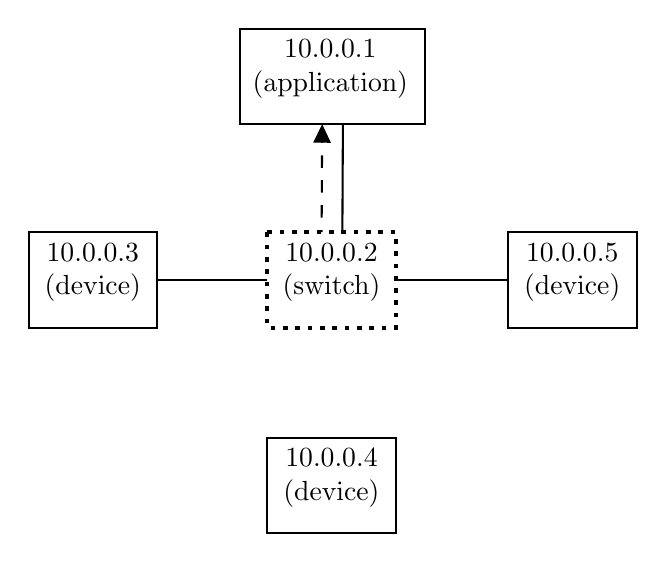
\begin{tikzpicture}[x=0.75pt,y=0.75pt,yscale=-1.0,xscale=1.0]
    %uncomment if require: \path (0,275); %set diagram left start at 0, and has height of 275
    
    
    % Text Node
    \draw    (123,15) -- (212,15) -- (212,61) -- (123,61) -- cycle  ;
    \draw (126,19) node [anchor=north west][inner sep=0.75pt]   [align=left] {\begin{minipage}[lt]{58.25pt}\setlength\topsep{0pt}
    \begin{center}
    10.0.0.1\\(application)
    \end{center}
    
    \end{minipage}};
    % Text Node
    \draw  [dash pattern={on 1.69pt off 2.76pt}][line width=1.5]   (136,113) -- (198,113) -- (198,159) -- (136,159) -- cycle  ;
    \draw (139,117) node [anchor=north west][inner sep=0.75pt]   [align=left] {\begin{minipage}[lt]{39.55pt}\setlength\topsep{0pt}
    \begin{center}
    10.0.0.2\\(switch)
    \end{center}
    
    \end{minipage}};
    % Text Node
    \draw    (21,113) -- (83,113) -- (83,159) -- (21,159) -- cycle  ;
    \draw (24,117) node [anchor=north west][inner sep=0.75pt]   [align=left] {\begin{minipage}[lt]{39.55pt}\setlength\topsep{0pt}
    \begin{center}
    10.0.0.3\\(device)
    \end{center}
    
    \end{minipage}};
    % Text Node
    \draw    (136,212) -- (198,212) -- (198,258) -- (136,258) -- cycle  ;
    \draw (139,216) node [anchor=north west][inner sep=0.75pt]   [align=left] {\begin{minipage}[lt]{39.55pt}\setlength\topsep{0pt}
    \begin{center}
    10.0.0.4\\(device)
    \end{center}
    
    \end{minipage}};
    % Text Node
    \draw    (252,113) -- (314,113) -- (314,159) -- (252,159) -- cycle  ;
    \draw (255,117) node [anchor=north west][inner sep=0.75pt]   [align=left] {\begin{minipage}[lt]{39.55pt}\setlength\topsep{0pt}
    \begin{center}
    10.0.0.5\\(device)
    \end{center}
    
    \end{minipage}};
    % Connection
    \draw    (172.38,61) -- (172.12,113) ;
    % Connection
    \draw    (198,136) -- (252,136) ;
    % Connection
    \draw    (136,136) -- (83,136) ;
    % Connection
    \draw  [dash pattern={on 4.5pt off 4.5pt}]  (162.37,64) -- (162.12,113) ;
    \draw [shift={(162.38,61)}, rotate = 90.29] [fill={rgb, 255:red, 0; green, 0; blue, 0 }  ][line width=0.08]  [draw opacity=0] (8.93,-4.29) -- (0,0) -- (8.93,4.29) -- cycle    ;
\end{tikzpicture}
\end{center}
\caption{Communication is marked as an arrow, scanned devices are highlighted.}
\label{Figure:NetworkDeviceRemove}
\end{figure}
